\chapter{Example: Numerical Integration}

In this chapter, we will look at a numerical computing problem that is well
suited to being parallelised, namely to calculate an approximation of a definite
integral:
\[
\int_a^b f(x) \, dx .
\]

%%%%%

\section{The Trapezium Rule}

The trapezium rule is a standard numerical technique to approximate the value
of an integral.  It splits the integral's range $[a,b]$ into $n \ge 1$
intervals:
\[\mstyle
\begin{align}
[{a+i\delta}, a+(i+1)\delta], 
  \quad\mbox{for $i = 0, \ldots, n-1$,} \\
\mbox{where $\delta = (b-a)/n$.}
\end{align}
\]
This is illustrated in Figure~\ref{fig:trapezium} with $n = 4$
(although in practice we would use a much larger value of~$n$).

%%%%%%%%%%%%%%%%

\begin{figure}
\begin{center}
\def\labY{-0.16}
\def\fn{\x^3/240 + \x^2/10 - 0.5*\x + 1.5}   %2.5*\x^2-2*\x+15}
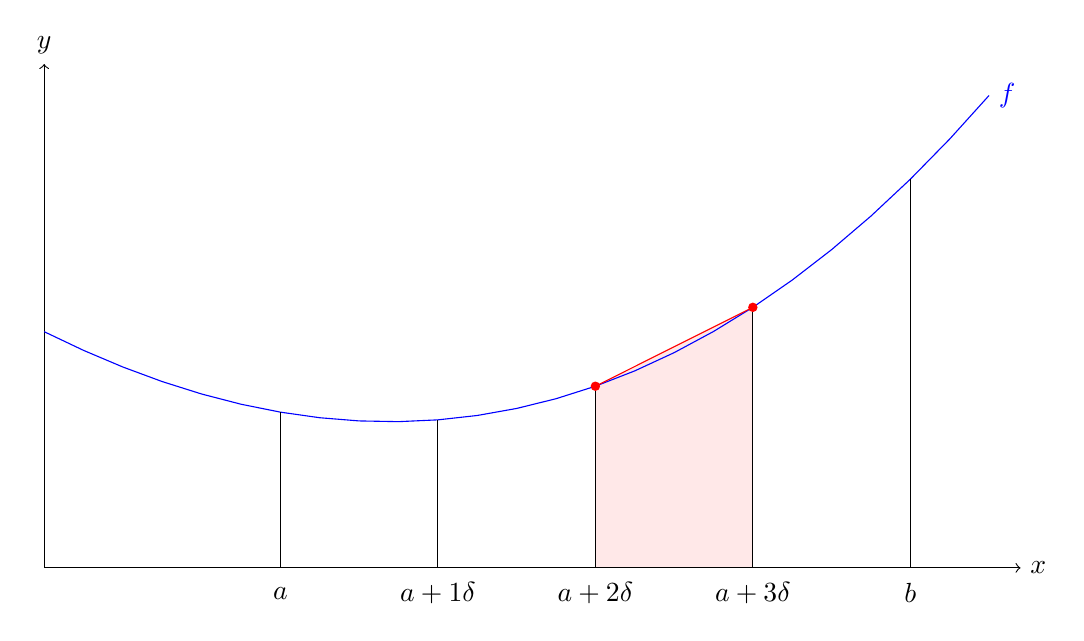
\begin{tikzpicture}[domain=0:6, scale = 2]
% Coordinates of selected points
\foreach \x in {3.5}  \draw (\x,\fn) coordinate (c1); %  node (c1) {};
\foreach \x in {4.5}  \draw (\x,\fn) coordinate (c2) {};
% Fill trapezium
\fill[red!9] (c1) -- (c2) -- (4.5,0) -- (3.5,0) -- (c1);
% Axes
\draw[->] (0,0) -- (6.2,0) node[right] {$x$};
\draw[->] (0,0) -- (0,3.2) node[above] {$y$};
% Plot
\draw[color=blue] plot (\x,\fn) node[right] {$f$}; 
% x labels
\draw(1.5,\labY) node{$a$};
\foreach \x in {1,2,3} \draw (\x+1.5,\labY) node{$a+\x \delta$};
\draw (5.5,\labY) node{$b$};
% Verticals
%\foreach \i in {0,1,2,3,4} \foreach \x in {\i+1.5} 
\foreach \x in {1.5,2.5,3.5,4.5,5.5} 
  \draw (\x,0) -- (\x,\fn);
% Blobs at selected points, and line between them
\draw[red] (c1) -- (c2);
\fill[red] (c1) circle[radius = 0.3mm];
\fill[red] (c2) circle[radius = 0.3mm];
\end{tikzpicture}
\end{center}
\caption{Illustration of the trapezium rule}
\label{fig:trapezium}
\end{figure}

%%%%%

The integral over the interval $[a+i\delta, a+(i+1)\delta]$ can then be
approximated by 
\[\mstyle
\frac{f(a+i\delta)+f(a+(i+1)\delta)}{2} * \delta.
\]
In other words, we approximate the graph of the function over this interval by
a straight line between the endpoints.  This is illustrated in
Figure~\ref{fig:trapezium} for the interval $[a+2\delta, a+3\delta]$.  The red
blobs give the values of the function at the endpoints; the function is
approximated by the red line; and so the integral is approximated by the area
of the pink region.  For this interval, the approach gives a slight
underapproximation. 

Summing over all intervals then gives us the following approximation:
\begin{eqnarray*}
\int_a^b f(x) \, dx  & \approx & 
  \left( \frac{f(a)+f(b)}{2} + \sum_{i=1}^{n-1} f(a+i\delta) \right) * \delta.
\end{eqnarray*}

Figure~\ref{fig:trapezium-sequential} gives straightforward sequential code to
implement the trapezium rule\footnote{The type {\scalashape Double
    \protect\SCALA{=>} Double} represents functions from {\scalashape Double}
  to {\scalashape Double}.}.  (We will see several implementations of the
trapezium rule, so we factor out some common code into an abstract class
|TrapeziumT|.)

%%%%%

\begin{figure}
\begin{scala}
/** Abstract class representing the problem of approximating the integral of £f£
  * from £a£ to £b£. */
abstract class TrapeziumT(f: Double => Double, a: Double, b: Double){
  /** Calculate the integral. */
  def apply(): Double

  /** Use trapezium rule to approximate the integral of £f£ from £left£ to £right£, 
    * using £n£ intervals of size £delta£. 
    * Precondition: £n*delta = right-left£ (modulo rounding errors). */
  protected 
  def integral(left: Double, right: Double, n: Int, delta: Double): Double = {
    require(n > 0 && Math.abs(n*delta-(right-left)) < 0.000000001) 
    var sum: Double=(f(right)+f(left))/2.0
    for(i <- 1 until n) sum += f(left+i*delta)
    sum*delta
  }
}

/** Approximation of the integral of £f£ from £a£ to £b£, using a sequential 
  * implementation of the trapezium rule. */
class SeqTrapezium(f: Double => Double, a: Double, b: Double, n: Int)
    extends TrapeziumT(f, a, b){
  require(n > 0)

  def apply() = integral(a, b, n, (b-a)/n)
}
\end{scala}
\caption{Sequential code to apply the trapezium rule.}
\label{fig:trapezium-sequential}
\end{figure}

%%%%%

\section{A parallel implementation}

Here's the idea of a parallel implementation.  We use some number |nWorkers|
of \emph{worker threads}.  We then split the interval $[a,b]$ into the same
number of equal-size sub-ranges, so each worker works on one sub-range.  A
\emph{controller} thread tells each worker which range to work on.  Each
worker sends its subresult back to the controller, which adds them up to give
the overall result.

This is a form of \emph{data parallelism}.  We split the data (the value
of~$f$ over the relevant range) between the workers.  Each worker calculates a
subresult on its part of the data, and then we combine the subresults. 

%% (This pattern is sometimes known as a \emph{farm}, and the controller as a
%% \emph{farmer}.) 

%%%%%

We will use a channel \SCALA{toWorkers} to communicate from the
controller to the workers, and a channel \SCALA{toController}
to communicate from the workers to the controller.  This is illustrated below.
%
\begin{center}
%\tikzstyle{every node}=[minimum width=5mm,minimum height = 15mm]
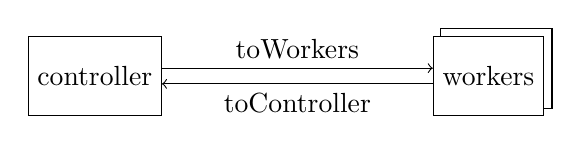
\begin{tikzpicture}
\draw (0,0) node[draw, minimum height = 10mm](c){\scalashape controller};
\draw (5,0) node[draw, minimum height = 10mm] (w){\scalashape workers};
\draw ([xshift = 1mm] w.north west) -- ++ (0,1mm) -- 
  ([xshift = 1mm, yshift = 1mm] w.north east) -- 
  ([xshift = 1mm, yshift = 1mm] w.south east) -- 
  ([yshift = 1mm] w.south east) ;
\draw[->] ([yshift = 1mm] c.east) -- node[above]{\scalashape toWorkers} 
  ([yshift = 1mm] w.west);
\draw[<-] ([yshift = -1mm] c.east) -- node[below]{\scalashape toController} 
  ([yshift = -1mm] w.west);
\end{tikzpicture}
\end{center}

In examples so far, each channel has had one sender and one receiver.
However, an in-port or out-port may be shared between any number of receivers
or senders.  Here, it is useful for the controller to use a single channel to
send to all the workers, and likewise to use a single channel to receive
subresults from all the workers.

Figure~\ref{fig:trapezium-1} gives some of the code.  The companion object
|Trapezium| factors out some definitions that we will reuse in a later
implementation. 

%%%%%

\begin{figure}
\begin{scala}
/** Companion object, collecting some code that is common across 
  * implementations. */
object Trapezium{
  /** Type of tasks to send to client.  The Task £(left, right, taskSize, delta)£
    * represents the task of calculating the integral from £left£ to £right£,
    * using £taskSize£ intervals of size £delta£. */
  type Task = (Double, Double, Int, Double)

  /** Make a channel, based on the value of `buffering`. */
  def mkChan[A: scala.reflect.ClassTag](buffering: Int): Chan[A] = 
    if(buffering == 0) new SyncChan[A] 
    else if(buffering == 1) new OnePlaceBuffChan[A]
    else if(buffering > 1) new BuffChan[A](buffering) 
    else new UnboundedBuffChan[A]
}

/** Parallel implementation of the trapezium rule. */
class Trapezium(
  f: Double => Double, a: Double, b: Double, n: Long, nWorkers: Int, buffering: Int = 0)
    extends TrapeziumT(f, a, b){
  require(n >= nWorkers)

  import Trapezium.{Task, mkChan}

  /** Channel from the controller to the workers, to distribute tasks. */
  private val toWorkers: Chan[Task] = mkChan[Task](buffering)

  /** Channel from the workers to the controller, to return sub-results. */
  private val toController: Chan[Double] = mkChan[Double](buffering)

  /** A worker, which receives arguments from the controller, estimates the
    * integral, and returns the results. */
  private def worker = thread("worker"){
    val (left, right, taskSize, delta) = toWorkers?()
    val result = integral(left, right, taskSize, delta)
    toController!result
  }

  ...
}
\end{scala}
\caption{Parallel implementation of the trapezium rule (part 1).}
\label{fig:trapezium-1}
\end{figure}

%%%%%

We want to experiment to see whether using buffered channels is advantageous.
We use the function~|mkChan| to make a channel passing data of type~|A|, where
the parameter |buffering| indicates the amount of buffering (with |0|
indicating a synchronous channel, and a negative value indicating an unbounded
buffered channel).

The controller needs to tell each worker the range \SCALA{[l,r]} to work on,
the number \SCALA{taskSize} of intervals in its range, and the size
\SCALA{delta} of each interval (so $\sm{taskSize} \times \sm{delta} \approx
\sm{r} - \sm{l}$).  We can pass this information as a 4-tuple \SCALA{(l, r,
  taskSize, delta)}.  We define a type |Task| to represent such 4-tuples, and
a channel |toWorkers| to pass |Task|s.

Each worker returns a \SCALA{Double} to the controller, so we define a channel
|toController| to pass such values.

The definition of a worker is then straightforward: it receives a task on the
|toWorkers| channel; calculates the approximation to the integral; and sends
the result back on the |toController| channel.

%%%%%

\begin{figure}
\begin{scala}
  /** This variable ends up holding the result. */
  private var result = 0.0

  /** A controller, who distributes tasks to the clients, and accumulates the
    * sub-results into £result£. */
  private def controller = thread("controller"){
    val delta = (b-a)/n    // Size of each interval.
    var remainingIntervals = n    // Number of intervals not yet allocated.
    var left = a // Left-hand boundary of the next task.
    for(i <- 0 until nWorkers){
      // Number of intervals in the next task; £$\lceil \sm{remainingIntervals/(nWorkers-i)} \rceil$£.
      val taskSize = ((remainingIntervals-1) / (nWorkers-i) + 1).toInt
      remainingIntervals -= taskSize; val right = left+taskSize*delta
      toWorkers!(left, right, taskSize, delta); left = right
    }

    // Receive results, and add them up.
    result = 0.0
    for(i <- 0 until nWorkers) result += toController?()
  }    
    
  /** The main system. */
  private def system = {
    val workers = || (for (i <- 0 until nWorkers) yield worker)
    workers || controller
  }

  /** Calculate the integral, and return the result. */
  def apply(): Double = { run(system); result } 
\end{scala}
\caption{Parallel implementation of the trapezium rule (part 2).}
\label{fig:trapezium-2}
\end{figure}

%%%%% Controller

We now consider the controller (given in Figure~\ref{fig:trapezium-2}).  We do
not assume that |n| (the number of intervals) is divisible by |nWorkers| (the
number of workers); instead, workers might receive slightly different size
tasks (but differing by at most one interval).  More precisely, the code
maintains a variable |remainingIntervals| that represents the number of
intervals still to allocate.  In the first loop, |nWorkers-i| represents the
number of tasks to send.  Then the next task contains $\lceil
\sm{remainingIntervals/(nWorkers-i)} \rceil$ intervals, i.e.~rounding up the
average (the expression defining |taskSize| calculates this using integer
arithmetic; the ``|/|'' is integer division; the final ``|toInt|'' is
necessary only because we took |n| to be a |Long|, and so the result of the
division is also a |Long|).

The second loop in the controller receives subresults from the workers, 
and accumulates them into the object variable |result|.

The function |system| constructs the system.  The definition of |workers|
builds a sequence of worker threads using a |for| expression (see Scala
box~\ref{sb:for-expression}).  It then combines them together in parallel
using an indexed form of parallel composition: if |ts| is a sequence of
|ThreadGroup|s, then \SCALA{\|\| ts} represents their parallel composition.

\framebox{for expressions}

Finally, the |apply| function runs the system and returns the final result
from the |result| variable. 

%%%%%%%%%%

\section{Testing}

We now consider how to test the concurrent implementation.  The obvious
approach is to run both the sequential and concurrent implementations on the
same integral, and test whether they give the same result.  In particular, my
approach was to generate random polynomials for the function~|f| to integrate,
and random values for |a|, |b|, |n| and |numWorkers| (within sensible ranges).

%%  (This assumes the sequential implementation is correct.)
However, it turns out that this approach doesn't quite work.  If we use both
implementations to approximate $\int_0^3 x^2 \mbox{d}x$ using $100$ intervals,
the sequential algorithm always gives
\[\mstyle
  9.000449999999995.
\]
However,  the concurrent implementation with 10 workers normally gives
\[\mstyle
  9.000449999999999,
\]
but sometimes gives
\[\mstyle
  9.000449999999997.
\]

%% \begin{quote}
%%   9.000449999999999
%%   9.000449999999997
%%   9.000449999999999
%%   9.000449999999999
%%   9.000449999999997 
%% \end{quote}

%%%%%


The difference in results can be explained by rounding errors, and in
particular that machine addition is not associative (you can verify this by
getting Scala to evaluate the expressions |(1E10 + (-1E10)) + 1E-10| and
\SCALA{1E10 + (-1E10 + 1E-10)}: the former gives the expected result, but the
latter evaluates to |0.0|, because rounding errors cause the final term to be
lost). 
%
In the sequential algorithm, the values for the intervals are added up from
left to right.  But in the concurrent algorithm, they are added up in a
different order, giving a different result.  Further, in different runs of the
concurrent algorithm, the sub-results are returned to the controller in
different orders, and so added up in different orders, giving different
results.

%%%%%

Instead, we can compare whether sequential result |seqResult| and the
concurrent result |concResult| are approximately equal using a test such as
\begin{scala}
assert(
  seqResult != 0.0 && Math.abs((seqResult-concResult)/seqResult) < 1E-7 ||
    Math.abs(seqResult-concResult) < 1E-10, ...)
\end{scala}
%
The second clause tests whether the relative result is less than one part in
$10^7$; the first clause guards against division by~$0$; the third clause is
necessary to cover the case where both the sequential and concurrent results
are small, the relative error isn't quite small enough to satisfy the second
clause, but the absolute error is very small.  (I originally omitted the third
clause, but one test produced a false error.) 

We can then run many such tests.

Incidentally, when I first ran these tests, they threw up other false errors,
because I hadn't thought carefully enough about preconditions of different
parts of the code.  For example, I hadn't realised that the |integral|
function (Figure~\ref{fig:trapezium-sequential}) requires a precondition
\SCALA{n > 0} (or else it gives an incorrect result); and hence the |Trapezium|
class (Figure~\ref{fig:trapezium-1}) requires a precondition |n >= nWorkers|
(or else a worker will receive an empty task).  
 % up to testing
\begin{slide}
\heading{Tuning}

We want to tune the program to run quickly.  There are two questions to
consider: 
%
\begin{itemize}
\item How many workers should we use?

\item Should we use buffered channels?
\end{itemize}
%
We can run some experiments to try to obtain (at least) partial answers to
these; although the answers are likely to vary with the architecture.

We consider $n$ (the number of intervals) as an input: under different
circumstances, we might want to use different values for~$n$.

%% Each experiment was as follows:
%% %
%% \begin{itemize}
%% \item The experiments were run on a 32-core server (two 2.1GHz Intel(R)
%% Xeon(R) E5-2683 CPUs with hyperthreading enabled).

%% \item 
%% Each instance estimated $\int_{-100000}^{+100000} x^2 \cos x \, \mbox{d}x$.
%% \end{itemize}

\end{slide}

%%%%%

\begin{slide}
\heading{How many workers to use?}

The experiments to decide the number of workers were as follows.
%
\begin{itemize}
\item The experiments were run on a 32-core server (two 2.1GHz Intel(R)
Xeon(R) E5-2683 CPUs with hyperthreading enabled).

\item 
Each instance calculated an approximation of $\int_{-100000}^{+100000} x^2
\cos x \, \mbox{d}x$.

\item
Various different sizes of $n$ were used between $2^{16}$ and $2^{28}$; each
observation calculated the integral $2^{28}/n$ times (so all observations were
about the same amount of work).

\item
Each instance used buffered channels with capacity 16.

\item
For each choice of $n$, various values of |nWorkers| were used.

\item
For each choice of parameters, multiple observations were made, and the mean
and 95\% confidence interval calculated.
\end{itemize}
\end{slide}

%%%%%

\begin{slide}
\label{slide:not-bag-of-tasks}
% scala -cp .:/home/gavinl/Scala/SCL:/home/gavinl/Scala/Util
% TrapeziumExperiment  --buffering 16 --doLog --strict --server on casteret
\begin{tikzpicture}
\begin{semilogxaxis}[
%  title = Timing experiment on the numerical integration example,
  ylabel = Time (ms),
  legend pos = north west,
  height = 0.98\textheight,
  width = 0.98\textwidth,
  scaled ticks = false,
  xlabel = Number of workers,
  xmin = 1,
  ymin = 0,
  ymax = 12000,
  log basis x=2
]

\addplot+[error bars/.cd, y dir=both,y explicit] coordinates {
  (512,66906.464174) +- (0,92.47266334851669)
  (256,33389.1291968) +- (0,90.82336557462699)
  (128,15921.3202264) +- (0,49.98543102984851)
  (64,7039.0096576000005) +- (0,50.23851632801305)
  (32,3477.035578181818) +- (0,31.78185210316302)
  (16,2806.8691438) +- (0,24.312484048502558)
  (8,2615.551757) +- (0,18.93106961242095)
  (4,3302.8918018000004) +- (0,21.88235727705309)
  (2,4821.4516514) +- (0,46.02325040305744)
  (1,8514.2120288) +- (0,30.33328457227989)
};
\addlegendentry{$n = 2^{18}$}
\addplot+[error bars/.cd, y dir=both,y explicit] coordinates {
  (512,17062.1814972) +- (0,68.81735222663036)
  (256,8716.506757) +- (0,73.74487896789209)
  (128,4338.5419785) +- (0,38.49607339998644)
  (64,2222.2029872) +- (0,21.052171978571973)
  (32,1620.89841275) +- (0,15.931547998759857)
  (16,1630.0650955714286) +- (0,15.321734270700714)
  (8,1902.2857148666665) +- (0,18.62486316909343)
  (4,2650.8328705999998) +- (0,19.107720313879742)
  (2,4337.412955571428) +- (0,36.724920562987535)
  (1,8001.85438) +- (0,73.38146511824169)
};
\addlegendentry{$n = 2^{20}$}
\addplot+[error bars/.cd, y dir=both,y explicit] coordinates {
  (512,1799.56714182) +- (0,32.71738180547917)
  (256,1363.52716338) +- (0,39.90186193386462)
  (128,1095.88527242) +- (0,33.988211371512506)
  (64,1038.1909207200001) +- (0,28.514381918295427)
  (32,1165.1984182) +- (0,16.087338188183626)
  (16,1249.4601490975608) +- (0,12.464870189761749)
  (8,1547.3894196666668) +- (0,15.351279424345195)
  (4,2433.725179540541) +- (0,24.262446412878784)
  (2,4060.8616351428573) +- (0,37.160363653690204)
  (1,7721.093534600001) +- (0,16.821275428807958)
};
\addlegendentry{$n = 2^{24}$}
\addplot+[error bars/.cd, y dir=both,y explicit] coordinates {
  (512,750.88449698) +- (0,54.81655513026725)
  (256,727.05934538) +- (0,56.4422401788819)
  (128,567.22785174) +- (0,24.78672447780806)
  (64,635.40388552) +- (0,7.342797598787894)
  (32,869.5884367346939) +- (0,8.678497290894436)
  (16,1047.3327939666667) +- (0,10.130131408714377)
  (8,1415.1987063333333) +- (0,10.95248597983864)
  (4,2292.3979252) +- (0,22.12424125790701)
  (2,4020.0490038125) +- (0,39.83178459400462)
  (1,7704.456190600001) +- (0,46.48908448403518)
};
\addlegendentry{$n = 2^{28}$}

\end{semilogxaxis}
\end{tikzpicture}
\end{slide}

%%%%%

\begin{slide}
\heading{Discussion of results}


\begin{itemize}
\item The amount of computation each worker performs is $O(1/\sm{nWorkers})$.
  But the amount of communication grows as $O(\sm{nWorkers})$.  

\item Each of the plots initially falls roughly proportional to
$1/\sm{nWorkers}$, which is proportional to $\sm{taskSize}$, i.e.~the
per-thread computation time.  

\item For larger values of |nWorkers|, the graphs seem to grow roughly
  proportional to |nWorkers|: the communication costs dominate.

%% The plots don't fall quite this quickly because
%% the communication and thread initialisation overheads grow proportional to
%% |nWorkers|.
\end{itemize}
\end{slide}

%%%%%


\begin{slide}
\heading{Discussion of results}

\begin{itemize}
\item
For small values of $n$ (up to about $2^{20}$), the optimal number of workers
is \emph{less} than the number of machine threads.  

Informal profiling with $n = 2^{18}$ and 64 workers shows that each worker
spends less than 25\% of its time calculating the integral: most of its
time is spent waiting for a task or waiting to send its result back to the
controller.
% scala -cp .:/home/gavinl/Scala/SCL:/home/gavinl/Scala/Util TrapeziumRun -p  64 --profile --reps 100 --size 262144 --buffering 16


The extra computation is dwarfed by the communication overheads. 

%% Extra threads reduce the per-thread computation time; but this is out-weighed
%% by the thread-creation and communication overheads.  In addition, the
%% controller acts as a bottleneck.

%% Beyond the optimal point, performance falls off rapidly: the thread-creation
%% and communication overheads dominate, and these are proportional to the number
%% of threads. 

\item
For larger values of $n$, the optimal number of workers is \emph{more} than
the number of machine threads (although the graphs are quite flat in this
range).  

Having more program threads than machine threads seems to give the
scheduler more chance for load balancing (rather like the pattern we will
look at in the next chapter). 
\end{itemize}
\end{slide}

%%%%%

\begin{slide}
\heading{Experiment concerning buffering}

We can carry out a similar experiment concerning the amount of buffering.
Some details:
%
\begin{itemize}
\item Various different sizes of $n$;

\item 64 worker threads;

\item Different amounts of buffering, including 0 (i.e.~a synchronous
  channel);

\item Other details as for the previous experiment.
\end{itemize}
\end{slide}

%%%%%


\begin{slide}
\begin{tikzpicture}
\begin{axis}[
%  title = Timing experiment on the numerical integration example,
  ylabel = Time (ms),
  legend pos = north east,
  height = 0.98\textheight,
  width = 0.98\textwidth,
  scaled ticks = false,
  %title = Experiment on the benefits of buffering,
  xlabel = Amount of buffering,
  xtick = data,
  ymax = 11500,
  symbolic x coords={0,1,2,4,8,16,32}
]

\addplot+[error bars/.cd, y dir=both,y explicit] coordinates {
  (0,8462.2592822) +- (0,71.8291716679859)
  (1,8717.5518986) +- (0,32.28246028517993)
  (2,7689.2159128) +- (0,31.958312511547966)
  (4,7290.773049) +- (0,28.02600837313684)
  (8,7121.698379) +- (0,70.10106910486228)
  (16,7048.133494) +- (0,37.00548631123019)
  (32,6916.198846125) +- (0,64.53008461366746)
};
\addlegendentry{$n = 2^{18}$}
\addplot+[error bars/.cd, y dir=both,y explicit] coordinates {
  (0,4388.0311806) +- (0,27.475385173157168)
  (1,4513.1778408) +- (0,34.95224329689597)
  (2,4018.3056444) +- (0,22.21917457523661)
  (4,3841.9693617142857) +- (0,37.030434873587765)
  (8,3768.1721822222225) +- (0,33.526125808993356)
  (16,3727.4166588000003) +- (0,32.77761738824269)
  (32,3702.6007) +- (0,37.01246780279705)
};
\addlegendentry{$n = 2^{19}$}
\addplot+[error bars/.cd, y dir=both,y explicit] coordinates {
  (0,2404.4758175) +- (0,22.94106417902077)
  (1,2461.1475072) +- (0,19.04718780190071)
  (2,2276.848227) +- (0,22.250667405164858)
  (4,2216.0773136) +- (0,22.09684430334622)
  (8,2189.798469625) +- (0,20.47038679802501)
  (16,2206.429703) +- (0,15.65965855716555)
  (32,2266.3921270833334) +- (0,21.966347711391997)
};
\addlegendentry{$n = 2^{20}$}
\addplot+[error bars/.cd, y dir=both,y explicit] coordinates {
  (0,1059.8903366) +- (0,28.944775149177275)
  (1,1057.9314238) +- (0,27.07197317361198)
  (2,1043.571615) +- (0,24.609794293852193)
  (4,1029.2399809199999) +- (0,29.75125397171397)
  (8,1032.20156518) +- (0,25.80973578121811)
  (16,1043.7603336) +- (0,24.16949383797133)
  (32,1041.58398964) +- (0,25.55474698045765)
};
\addlegendentry{$n = 2^{24}$}

\end{axis}
\end{tikzpicture}
\end{slide}

%%%%%

\begin{slide}
\heading{Discussion of results}

Buffering helps for examples with more workers than the optimal number (for
the given~$n$).  Curiously, buffering of size~1 makes things slower, however.

For examples with a more appropriate number of workers (for the given~$n$),
buffering makes very little difference, in this case.  However, it might make
more difference in other examples, particularly where the time to produce and/or
process a task is more variable.
\end{slide}

% \begin{slide}
% \heading{Experimental results}

% The following table shows the time taken (in ms) to run the system, with
% \SCALA{n=63000}, on an 8 processor machine, with Just In Time compilation
% turned \emph{off} (averaged over 200 runs).
% %
% \begin{trivlist}\item[]\def\tabcolsep{1.7mm}
% \begin{tabular}{*{19}{c}}
% nWorkers: & 1 & 2 & 3 & 4 & 5 & 6 & 7 & 8 & 9 & 10 & 12 & 15 & 20\\
% time: & 165 & 108 & 85 & 70 & 60 & 55 & 52 & 51 & 59 & 59 & 55 & 52 & 51\\[2mm]
% \end{tabular}
% \end{trivlist}

% How can we explain the figures?
% \end{slide}

% %%%%%

% \begin{selfnote}
% The fastest is when each worker is on a separate processor.  (In this case the
% controller doesn't do much work.  In an example where the controller does a
% lot of work, the fastest might be when the $\# workers = \# processors - 1$.) 

% In an ideal world, it would be $1/nWorkers$ for $nWorkers \le 8$.  But there's an
% overhead, both per extra process and overall.

% Once $nWorkers > 8$, the processes have to compete for the processors, and the
% extra time for the context switches makes it slower overall.

% I don't really understand why it gets faster again for 15 and 20.
% \end{selfnote}

%% n = 630000, 100 times each, JIT off

%% nWorkers = 1      Time taken: 156.061
%% nWorkers = 2      Time taken: 109.354
%% nWorkers = 3      Time taken: 87.591
%% nWorkers = 4      Time taken: 70.119
%% nWorkers = 5      Time taken: 60.185
%% nWorkers = 6      Time taken: 55.064
%% nWorkers = 7      Time taken: 52.063
%% nWorkers = 8      Time taken: 51.971
%% nWorkers = 9      Time taken: 56.148
%% nWorkers = 10     Time taken: 58.047
%% nWorkers = 12     Time taken: 59.018
%% nWorkers = 15     Time taken: 56.04
%% nWorkers = 20     Time taken: 57.163

%%%%%

% \begin{slide}
% \heading{Experimental results}

% The following table shows the time taken (in ms) to run the system, with
% \SCALA{n=1260000} (20 times more than the previous experiment), on the same
% machine, with Just In Time compilation turned \emph{on} (again averaged over
% 200 runs).
% %
% \begin{trivlist}\item[]\def\tabcolsep{1.5mm}%
% \begin{tabular}{*{19}{c}}
% nWorkers: & 1 & 2 & 3 & 4 & 5 & 6 & 7 & 8  & 9 & 10 & 12 & 15 & 20 \\
% time:  & 152 & 157 & 134 & 117 &  100 & 80 & 74 & 69 & 63 & 64 & 64 & 65 & 67
% % time:   & 76 & 79 & 64 & 56 & 48 & 43 & 39 & 37 & 37 & 36 & 37 & 37 & 39
% \end{tabular}
% \end{trivlist}
% %
% The Just In Time compilation has an odd effect!
% \end{slide}

% %%%%%

% \begin{slide}
% \heading{Comments}

% In this case, we could have constructed the workers with the
% appropriate values for \SCALA{f, l, r, taskSize, delta}, rather than having the
% controller distribute them.  However, we wanted to illustrate the
% pattern of having a controller distribute work to the workers.
% \end{slide}

%%%%%
 % experiments
\section{The Bag-of-Tasks Pattern}

In the previous sections, we chose to distribute the work equally between the
workers.
%
This is sensible if each worker will be executed on its own processor,
all the processors are the same speed, all are equally loaded with other
tasks, and it's possible to identify what an equal distribution is.
%
But in many cases, not all of these things will be true.

An alternative is to use smaller tasks, with more tasks than workers.  
%
In the numerical integration example, each task will be to estimate the
integral over some subrange.   We use \SCALA{nTasks} tasks, where
$\sm{nTasks} \ge \sm{nWorkers}$.
%
The tasks are distributed between the workers, each receiving a new task when
it has finished the previous one.  In this way, the faster workers will
complete more tasks than the slower ones, which provides for a form of load
balancing.

This pattern is known as \emph{bag of tasks}: the controller holds a bag of
tasks, which it distributes to workers.  (Sometimes workers return sub-tasks
to the controller, but that's not the case here.)

%%%%%

Most of the code to apply the bag-of-tasks pattern to the numerical
integration example is in Figure~\ref{fig:bag-of-tasks}.  (We omit code that
is essentially identical to earlier.)

Adapting the definition of a worker is straightforward.  Each worker thread
repeatedly receives and processes tasks, keeping track of the sum of the
estimates it has calculated so far.  
%
The controller closes the |toWorkers| channel to indicate that there are no
remaining tasks, at which point the worker sends its total to the controller.
%
An alternative would be to send the subresult for each task to the controller
immediately; however, that would lead to more channel communications, so is
likely to be slower.

%%%%%%%%%%%%%%%%%%%%%%%%

\begin{figure}
\begin{scala}
  private def worker = thread("worker"){
    var myTotal = 0.0
    repeat{
      val (left, right, taskSize, delta) = toWorkers?()
      myTotal += integral(left, right, taskSize, delta)
    }
    toController!myTotal
  }

  private def distributor = thread("distributor"){
    val delta = (b-a)/n    // Size of each interval.
    var remainingIntervals = n    // Number of intervals not yet allocated.
    var left = a // Left-hand boundary of next task.
    for(i <- 0 until nTasks){
      // Number of intervals in the next task; £$\lceil \sm{remainingIntervals}/(\sm{nTasks}-\sm i)\rceil$£.
      val taskSize = ((remainingIntervals-1) / (nTasks-i) + 1).toInt
      remainingIntervals -= taskSize; val right = left+taskSize*delta
      toWorkers!(left, right, taskSize, delta); left = right
    }
    toWorkers.endOfStream()
  }

  private var result = 0.0

  private def collector = thread("collector"){
    result = 0.0
    for(i <- 0 until nWorkers) result += toController?()
  }

  private def system = {
    val workers = || (for (i <- 0 until nWorkers) yield worker)
    workers || distributor || collector
  }

  def apply(): Double = { run(system); result } 
\end{scala}
\caption{The bag-of-tasks pattern applied to the numerical integration
  example.}
\label{fig:bag-of-tasks}
\end{figure}

%%%%%%%%%%


%%%%% \heading{The controller}

The controller has to both distribute tasks (on |toWorkers|), and receive
results (on |toController|).
%
We could implement this using a single controller thread.  This approach would
be reasonably straightforward in this case, because all the communications on
|toController| follow those on |toWorkers|.  However, in other examples the
communications over the different channels might be interleaved, which makes a
single-thread approach trickier.

The issues of distributing the tasks and receiving the results are
independent, so it is cleaner to separate them.  The easiest way to do this is
to use two concurrent threads, one for each aspect.  In some examples, this
might also give better performance, if the controller acts as a bottleneck.

We therefore build the controller as the composition of a distributor and a
collector, communicating with the workers as illustrated below.
%
\begin{center}
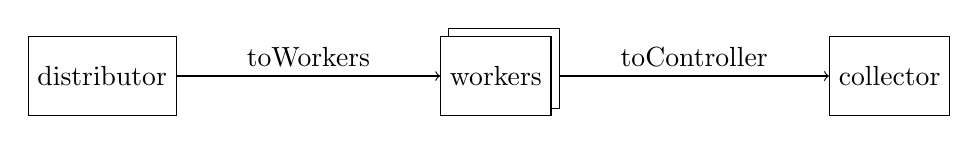
\begin{tikzpicture}
\draw (0,0) node[draw, minimum height = 10mm](d){\scalashape distributor};
\draw (5,0) node[draw, minimum height = 10mm] (w){\scalashape workers};
\draw ([xshift = 1mm] w.north west) -- ++ (0,1mm) -- 
  ([xshift = 1mm, yshift = 1mm] w.north east) -- 
  ([xshift = 1mm, yshift = 1mm] w.south east) -- 
  ([yshift = 1mm] w.south east) ;
\draw[->] (d) -- node[above]{\scalashape toWorkers}   (w);
%
\draw (10,0)  node[draw, minimum height = 10mm](c){\scalashape collector};
\draw[->] ([xshift = 1mm] w.east) -- node[above]{\scalashape toController} (c);
\end{tikzpicture}
\end{center}

%%%%%

The code for distributing the tasks is almost identical to earlier, except now
the distributor sends out |nTasks| tasks.  And the code for the collector is
identical to the relevant part of the previous controller. 

We then construct the system as illustrated above.  The resulting program can
be tested in the same way as for the previous implementation. 
 % bag of tasks
\subsection{Tuning experiments}

%%%%%

\begin{figure}
\begin{center}
\begin{tikzpicture}
\begin{semilogxaxis}[
%  title = Timing experiment on the numerical integration example,
  ylabel = Time (ms),
%  legend pos = north east,
  legend style={at={(0.70,0.98)}},
  height = 0.55\textheight,
  width = 0.85\textwidth,
  scaled ticks = false,
%  title = Experiment on the numerical integration bag-of-tasks example.,
  xlabel = Number of workers,
  log basis x=2,
  ymin = 500,
  ymax = 5000
]
\addplot+[error bars/.cd, y dir=both,y explicit] coordinates {
  (1,5450.6101748) +- (0,12.650706471088398)
  (2,3056.442098428571) +- (0,28.737642840384968)
  (4,2154.3953815666664) +- (0,20.693639090142195)
  (8,3350.65515325) +- (0,32.63665761213119)
  (16,5594.300504181818) +- (0,50.32486183690076)
  (32,7475.9241562) +- (0,48.417094704814176)
  (64,9986.346586285716) +- (0,98.09082844202608)
};
\addlegendentry{$\sm n = 2^{18}$, $\sm{nTasks} = 2^{9}$}
\addplot+[error bars/.cd, y dir=both,y explicit] coordinates {
  (1,5007.675461) +- (0,13.686326182482928)
  (2,2731.0204338333333) +- (0,23.35039731606894)
  (4,1616.8292285185184) +- (0,16.138829689738955)
  (8,1865.081054625) +- (0,18.53227480228986)
  (16,2701.604537571429) +- (0,25.969680061097936)
  (32,3680.565586090909) +- (0,36.210743908097214)
  (64,4568.203701666667) +- (0,41.715695160489254)
};
\addlegendentry{$\sm n = 2^{20}$; $\sm{nTasks} = 2^{10}$}
\addplot+[error bars/.cd, y dir=both,y explicit] coordinates {
  (1,4884.6682636000005) +- (0,17.782427429822622)
  (2,2570.123440777778) +- (0,24.80872494458182)
  (4,1514.0846481400001) +- (0,31.850239055539483)
  (8,1263.6072703599998) +- (0,29.581306649002393)
  (16,1628.5271092424243) +- (0,15.899583168616081)
  (32,2100.7852361428572) +- (0,20.340306504248268)
  (64,2461.952226961538) +- (0,23.696128463145246)
};
\addlegendentry{$\sm n = 2^{22}$; $\sm{nTasks} = 2^{11}$}
\addplot+[error bars/.cd, y dir=both,y explicit] coordinates {
  (1,4922.292719333333) +- (0,38.37834775822396)
  (2,2677.5306812) +- (0,24.85402705231822)
  (4,1538.3950354400001) +- (0,17.909341023643474)
  (8,1070.5430969400002) +- (0,34.3563713210201)
  (16,1133.5246862000001) +- (0,9.883390535725946)
  (32,1373.7130467380953) +- (0,13.717792332933353)
  (64,1626.3286156818183) +- (0,16.00981709292464)
};
\addlegendentry{$\sm n = 2^{24}$; $\sm{nTasks} = 2^{12}$}
\addplot+[error bars/.cd, y dir=both,y explicit] coordinates {
  (1,5069.178585542857) +- (0,50.37213086034046)
  (2,2691.89330344) +- (0,37.767455164393304)
  (4,1530.5242046600001) +- (0,28.817161707223033)
  (8,1010.6285473400001) +- (0,32.66829660709502)
  (16,1017.41061254) +- (0,30.678738953720778)
  (32,1084.9625646) +- (0,15.169669087395743)
  (64,1244.38884936) +- (0,12.978136074354166)
};
\addlegendentry{$\sm n = 2^{26}$; $\sm{nTasks} = 2^{13}$}
\end{semilogxaxis}
\end{tikzpicture}

\end{center}
\caption{Experiments on the bag-of-tasks example.}
\label{fig:bag-of-tasks-experiment}
\end{figure}

%%%%%

Figure~\ref{fig:bag-of-tasks-experiment} shows timing results for the
bag-of-tasks example.  Each plot considers a particular choice for the number
of intervals, |n|, and the number of tasks, |nTasks|.  The x-axis considers
different numbers of workers, and the y-axis gives the times taken.  Each run
used unbounded buffered channels.  Each observation performed $2^{27}/\sm{n}$
runs.

It is useful to consider the quantity $\sm n / \sm{nTasks}$ for each plot,
i.e.~the number of intervals per tasks, which runs from $2^9$ to $2^{13}$ by
factors of~$2$.  This is a good measure of the computational cost of each
task.   For smaller values of this measure, the program achieves poor scaling,
being slower for eight workers than for four.  This is consistent with what we
saw earlier: the low computational cost of each task means that the channels
become congested.  However, for higher values of this measure, the program
scales better.  

%%%%%

Figure~\ref{fig:bag-of-tasks-experiment-2} gives results for experiments
considering the number of tasks to give each worker.  Each run used eight
workers, and unbounded buffered channels.  Each plot considers a particular
value for the number of intervals,~|n|.  The x-axis gives the average number
of tasks per worker.  Each observation is based on $2^{28}/\sm{n}$ runs.

\begin{figure}
% scala  tacp.trapezium.TrapeziumExperiment --doBagNumTasks --strict
\begin{center}
\begin{tikzpicture}
\begin{semilogxaxis}[
%  title = Timing experiment on the numerical integration example,
  ylabel = Time (ms),
%  legend pos = north east,
  legend style={at={(0.55,0.98)}},
  height = 0.55\textheight,
  width = 0.85\textwidth,
  scaled ticks = false,
%  title = Experiment on the numerical integration bag-of-tasks example considering the number of tasks.,
  xlabel = Tasks per worker,
  log basis x=2,
  ymax = 3800
]
\addplot+[error bars/.cd, y dir=both,y explicit] coordinates {
  (1,3352.5584418666667) +- (0,32.39018336931468)
  (2,3177.6074104) +- (0,30.03046065403267)
  (4,2825.346039153846) +- (0,26.578742030652567)
  (8,2633.3589845416664) +- (0,26.058560420431323)
  (16,2556.6023542105263) +- (0,25.525369128045856)
  (32,2602.1325810999997) +- (0,25.620813091083203)
  (64,2754.1994305999997) +- (0,26.43581717528377)
  (128,3386.6708786) +- (0,26.598870170170244)
  (256,4947.1010282) +- (0,48.25750793782477)
};
\addlegendentry{$\sm n = 2^{20}$}
\addplot+[error bars/.cd, y dir=both,y explicit] coordinates {
  (1,2430.0985353076926) +- (0,24.161751494140365)
  (2,2590.3529583000004) +- (0,25.299756842425655)
  (4,2153.021478857143) +- (0,21.273131359790593)
  (8,1925.8373171666667) +- (0,17.959884614345665)
  (16,1836.6189299722223) +- (0,18.19037513122588)
  (32,1825.1809766071428) +- (0,18.10857316008791)
  (64,1839.26816146875) +- (0,18.20233464725214)
  (128,1880.6876090666667) +- (0,18.619059018086812)
  (256,2134.17022104) +- (0,28.68720991042429)
};
\addlegendentry{$\sm n = 2^{22}$}
\addplot+[error bars/.cd, y dir=both,y explicit] coordinates {
  (1,2049.76257738) +- (0,20.246850253890152)
  (2,2428.827615181818) +- (0,24.25034273533704)
  (4,1977.1314379230769) +- (0,19.558354330713257)
  (8,1686.9642632222224) +- (0,16.774562309432827)
  (16,1573.5973083611111) +- (0,15.678148981214)
  (32,1562.8593507857145) +- (0,15.444602885745132)
  (64,1570.87964412) +- (0,18.331970500511368)
  (128,1558.21264084) +- (0,22.30355302530338)
  (256,1691.5533438599998) +- (0,32.58672115299523)
};
\addlegendentry{$\sm n = 2^{24}$}
%% \addplot+[error bars/.cd, y dir=both,y explicit] coordinates {
%%   (1,1925.447759847826) +- (0,19.18777386975458)
%%   (2,2400.668871714286) +- (0,23.39996657676753)
%%   (4,1921.7963885384615) +- (0,19.058506647775467)
%%   (8,1652.4909764285715) +- (0,16.169790819327602)
%%   (16,1502.772550652174) +- (0,14.76747235535448)
%%   (32,1524.1503742999998) +- (0,14.118010595497367)
%%   (64,1522.0211753636363) +- (0,15.055364262187124)
%%   (128,1464.9243361666668) +- (0,14.226315577346861)
%%   (256,1581.72356702) +- (0,26.315896274033975)
%% };
%% \addlegendentry{$\sm n = 2^{26}$}
\addplot+[error bars/.cd, y dir=both,y explicit] coordinates {
  (1,1853.7602047799999) +- (0,23.20821176816953)
  (2,2337.0621846153845) +- (0,21.871343828100212)
  (4,1899.366764) +- (0,18.96852892309966)
  (8,1634.8610090999998) +- (0,24.11141714793872)
  (16,1501.6389951400001) +- (0,19.394279658177584)
  (32,1491.06709548) +- (0,17.686753672081153)
  (64,1490.079240175) +- (0,14.677187086601563)
  (128,1494.2455339795918) +- (0,14.746633258811613)
  (256,1525.11317254) +- (0,27.009019402748162)
};
\addlegendentry{$\sm n = 2^{28}$}
\end{semilogxaxis}
\end{tikzpicture}

\end{center}
\caption{Experiments on the bag-of-tasks example, considering the number of
  tasks per worker.}
\label{fig:bag-of-tasks-experiment-2}
\end{figure}

Each plot shows a decrease in time as the number of tasks per worker increases
from two to about sixteen.  Having more tasks allows for better load
balancing.  However, beyond a certain point, increasing the number of tasks
makes the program slower: at this point, the channel communication becomes a
bottleneck again.

Most of the plots show that using an average of two tasks per worker is slower
than just one, which may seem surprising.  I investigated this by arranging
for each worker to print the number of tasks it processed.  When the average
is one task per worker, it is nearly always the case that each worker indeed
executes exactly one task; the difference in times taken by workers is not
very large in this case.  However, when the average is two tasks per worker,
it is normally the case that at least one (slow) worker performs only one
task, and so another worker performs three; the latter worker therefore takes
considerably longer than the others, and this increases the overall running
time.

It is worth noting that each of the plots has a fairly wide U-shape.  For the
lower three plots, there is little difference between $2^4$ and $2^7$ tasks
per worker.  This is a good situation, as it suggests the program is fairly
stable with respect to changes in speed of workers, for example caused by
different hardware. 

Experiments on the 32-core server gave similar results, except in order to
benefit from the additional machine threads, each task needs to be larger, as
in Section~\ref{sec:trapezium-tuning}.

% \framebox{casteret}

 % experiments
\section{Encapsulation}
\label{sec:bag-of-tasks-encapsulation}

In the previous code, the design decisions concerning the use of
message-passing concurrency were interleaved with the computation itself.  If
we decided to implement the concurrency in a different way---for example, to
use one of the techniques we'll see later in the course---we would have to
change the code in several different places.  This is a very small program, so
it doesn't matter too much here; but it would be an issue in bigger programs.

It would be better to encapsulate each relevant design decision within a
single object, so that changes will involve just that object.  Each such
object will be designed to allow concurrent calls of its methods, and to avoid
race conditions.  

Further, reasoning about correctness will (mostly) involve reasoning about a
single object at a time: code outside that object can use it without worrying
about how it is implemented.  We will see this idea of encapsulation a lot
later in the book.  We will encapsulate a datatype---such as a queue or a
mapping---inside an object that provides thread-safe operations on the
datatype; code outside the object can mostly use the datatype in the same way
as in a sequential setting.  

%%%%%

For the example of this chapter, we will define concurrent objects with the
interfaces given in Figure~\ref{fig:BoT-interfaces}.  The |BagOfTasks| objects
have an operation to allow a worker thread to get a task.  We have made the
design decision to return the special value |null| in the case that there are
no more tasks.  An alternative would be to throw a |Stopped| exception, as
earlier; but using |null| seems cleaner, and is appropriate because |null| is
easily distinguished from a real task.  The |Collector| objects have an
operation to allow a worker to submit its final subtotal, and an operation to
get the overall total.

%%%%%%

\begin{figure}
\begin{scala}
  /** The bag-of-tasks object. */
  trait BagOfTasks{
    /** Get a task.  Returns £null£ if there are no more tasks. */
    def getTask(): Task 
  }  

  /** A collector object that combines subresults from the workers. */
  trait Collector{
    /** Add x to the result. */
    def add(x: Double) 

    /** Get the result, once the computation has finished. */
    def get: Double 
  }
\end{scala}
\caption{The interfaces for the bag-of-tasks and collector objects.}
\label{fig:BoT-interfaces}
\end{figure}

%%%%%

It is straightforward to adapt the definition of a worker to use such objects.
The definition is parameterised by the |BagOfTasks| and |Collector|.  It calls
the |getTask| operation on the |BagOfTasks| to get a task, exiting its main
loop when it receives |null|.  It then uses the |add| operation on the
|Collector| to return its subtotal.
%
\begin{mysamepage}
\begin{scala}
  private def worker(bag: BagOfTasks, collector: Collector) = thread("worker"){
    var myTotal = 0.0; var done = false
    while(!done) bag.getTask() match{
      case null => done = true
      case (left, right, taskSize, delta) =>
        myTotal += integral(left, right, taskSize, delta)
    }
    collector.add(myTotal)
  }
\end{scala}
\end{mysamepage}

Below we will define an implementation |BagOfTasksChannels| of |BagOfTasks|,
and an implementation |CollectorChannels| of |Collector|.  The main |apply|
method creates the two objects, runs the workers, and then gets the
final result from the collector.
\begin{scala}
  def apply(): Double = {
    val bag = new BagOfTasksChannels(a, b, n, nTasks, nWorkers, buffering)
    val collector = new CollectorChannels(nWorkers, buffering)
    val workers = || (for (i <- 0 until nWorkers) yield worker(bag, collector))
    run(workers)
    collector.get
  }
\end{scala}

%%%%%

An implementation of |BagOfTasks| using message passing is in
Figure~\ref{fig:bagOfTasksObject}.  This contains a server thread that sends
|Task|s on the private |toWorkers| channel.  Once all proper tasks have been
sent, it sends |null| multiple times, once for each worker.  A worker can
obtain a task (either a proper task or |null|) by receiving on |toWorkers|.
Note that |toWorkers| is a private channel within the object: this ensures
that client code can interact with the object only as intended.

%%%%%

\begin{figure}
\begin{scala}
class BagOfTasksChannels(
  a: Double, b: Double, n: Long, nTasks: Int, numWorkers: Int, buffering: Int)
    extends BagOfTasks{
  /** Channel from the server to the workers, to distribute tasks. */
  private val toWorkers = mkChan[Task](buffering)

  /** Get a task.  Return £null£ if there are no more tasks. */
  def getTask(): Task = toWorkers?() 

  /** A server process that distributes tasks. */
  private def server = thread("bag of tasks"){
    val delta = (b-a)/n; var remainingIntervals = n; var left = a
    for(i <- 0 until nTasks){
      val taskSize = ((remainingIntervals-1) / (nTasks-i) + 1).toInt
      remainingIntervals -= taskSize; val right = left+taskSize*delta
      toWorkers!(left, right, taskSize, delta); left = right
    }
    for(i <- 0 until numWorkers) toWorkers!null
  }

  fork(server)  // Start the server running.
}
\end{scala}
\caption{An implementation of {\scalashape BagOfTasks} using message passing.}
\label{fig:bagOfTasksObject}
\end{figure}

%%%%%

The server is started by the command |fork(server)|, which is executed as part
of the construction of the |BagOfTasksChannels| object.
%
More generally, if |t| is a |ThreadGroup|, then |fork(t)| or |t.fork| starts a
new thread (or threads) running which executes~|t|.  However---unlike with
|run(t)|---the new thread runs in parallel to the current thread.  In
Figure~\ref{fig:bagOfTasksObject}, the construction of the
|BagOfTasksChannels| object returns after the |fork(server)|, but leaves a
thread running the |server| code.

%%%%% \heading{Encapsulating the collector}

An implementation of |Collector| using message passing is in
Figure~\ref{fig:collector}.  This again contains a server thread, which is set
running as part of the construction of the object.  The |add(x)| method
sends~|x| to the server, which adds it to its running total.  The |get|
operation receives the final result from the server.

%%%%%

\begin{figure}
\begin{scala}
  private class CollectorChannels(buffering: Int) extends Collector{
    /** Channel from workers to the server. */
    private val toController = mkChan[Double](buffering)

    /** Channel that sends the final result. */
    private val resultChan = new SyncChan[Double]

    /** Add x to the result. */
    def add(x: Double) = toController!x

    /** Get the result. */
    def get: Double = resultChan?()
    
    /** A collector, that accumulates the subresults. */
    private def server = thread("collector"){
      var result = 0.0
      for(i <- 0 until nTasks) result += (toController?())
      resultChan!result
    }

    fork(server)    // Start the server running.
  }
\end{scala}
\caption{An implementation of {\scalashape Collector} using message passing.}
\label{fig:collector}
\end{figure}

%%%%%


There is a slight subtlety in the implementation of the collector.  Recall
that the main |apply| operation calls |get| after all the workers have
terminated.  It would be incorrect to make |result| an object variable, and
for the |get| method to just read that variable, because that would constitute
a race.  It is possible that the |server| thread has received a subtotal
from the final worker thread, but not yet added it to |result|, so the |apply|
operation would receive the wrong value!  With the code
in~\ref{fig:collector}, we can be sure that the correct value is sent: the
|get| operation is blocked until the server has received all the subtotals.

 % encapsulation 

%%%%%%%%%%%%%%%%%%%%%%%%%%%%%%%%%%%%%%%%%%%%%%%%%%%%%%%

\section{Summary}

In this chapter we have studied a data parallel problem.  The approach to such
problems is to split the input data between different worker threads, and to
combine the results together.  Many compute-intensive problems fall into this
class, so it is a very useful pattern.  It  requires that there is some
meaningful way to split the data between workers, and to combine the results
efficiently.

We arranged for a controller thread to distribute tasks to workers, using two
different approaches.  In the first approach, the controller sent each worker
a single task.  (In fact, in this case we could have included the task as a
parameter of the |worker| function; but we wanted to illustrate this technique
of distributing tasks.)  In the second approach, the bag of tasks, the
controller distributed multiple tasks to workers; this helped to balance the
load between workers, overcoming differences in speed.

We tested each implementation against a corresponding sequential algorithm.
This is a very common technique.  A wrinkle here is that rounding errors
caused the two algorithms to give slightly different results.  

We also ran experiments to understand how best to choose parameters such as
the number of workers and the number of tasks.  The main error one can make
here is to take tasks to be too small.  This leads to the channels becoming
bottlenecks, and the program being inefficient.  It can be best to run fewer
threads than the number of machine threads available, so as to avoid these
bottlenecks.  Each task should be large enough that workers spend nearly all
their time actually performing the tasks, as opposed to trying to send and
receive messages.  

%% \framebox{TO DO}

%% \begin{itemize}
%% %% \item
%% %% Data parallel;

%% %% \item
%% %% Workers and controllers;

%% %% \item
%% %% Closing channels;

%% %% \item
%% %% Testing against a sequential implementation;

%% \item
%% %% Choosing the number of processes and the amount of buffering;

%% %% \item
%% %% Beware of having too many communications: the channel will act as a bottleneck;

%% %% \item
%% %% Experimental design.

%% %% \item
%% %% Bag of tasks;

%% \item
%% Choosing the size of tasks;

%% \item
%% Communication is expensive: avoid having too many communications;

%% \item
%% Encapsulation;

%% %% \item Bag of tasks with replacement.
%% \end{itemize}

In Section~\ref{sec:bag-of-tasks-encapsulation}, we encapsulated the bag of
tasks and the collector inside objects.  This meant that we could concentrate
on that part of the implementation in isolation from other parts; and the
other parts of the program could use these objects without concern for how
they were implemented.  Further, this technique means that we could replace
those objects by other objects that produce the same external behaviour, but
perhaps using different concurrency techniques \framebox{forward ref here}.

Encapsulation like this will be an important theme in later chapters.  We will
arrange for nearly all of the concurrency to be encapsulated within such
objects.  This will make it much easier to justify correctness: local
correctness arguments that depend on a fairly small amount of code are easier
than global arguments that encompass a large program.  The correctness
property of such objects will be that the operation calls appear to take place
in a one-at-a-time order, without interfering with one another.

A variant on the bag-of-tasks pattern allows new tasks to be placed back into
the bag.  This can be the case where some tasks can be solved directly, but
other tasks lead to two or more recursive subtasks.  The latter case can be
tackled by returning subtasks to the bag.  We will need some extra machinery
to support returning tasks to the bag, which we will see in
Chapter~\ref{chap:alts}; exercises in that chapter investigate this technique.

%% \emph{Adaptive quadrature} is an alternative approach that proceeds as
%% follows.  In order to calculate the integral $\int_a^b f(x) \mbox{d}x$,
%% compute the midpoint $mid = (a+b)/2$ and estimate three integrals, from $a$ to
%% $mid$, from $mid$ to~$b$, and from $a$ to~$b$, each using the trapezium rule
%% with a single interval.  If the sum of the former two estimates is within some
%% value $\epsilon$ of the third, then we take that third estimate as being the
%% result.  Otherwise, recursively estimate the integrals over the two
%% sub-intervals $a$ to~$mid$ and $mid$ to~$b$, and sum the results.

%% The latter case can be implemented by returning the two sub-intervals $(a,
%% mid)$ and $(mid, b)$ to the bag.


%%%%%%%%%%%%%%%%%%%%%%%%%%%%%%%%%%%%%%%%%%%%%%%%%%%%%%%

\section*{Exercises}

\begin{questionS}
\begin{enumerate}
\item
Suppose $x$ and $y$ are random numbers, chosen with a uniform distribution on
$[0,1)$.  Show that the probability that $x^2+y^2 < 1.0$ is $\pi/4$.  Hint:
  use a geometric argument.

\item
Use this idea to write a concurrent program to estimate the value of $\pi$.
%% (You might use the class |scala.util.Random| to generate random numbers.) 

%% \item
%% (For those who have taken a course on probability:) Estimate the
%%   standard deviation of the results given by your program.
\end{enumerate}
\end{questionS}

%%%%%

\begin{answerS}
\begin{myminipage}{102mm}
For part (a), consider a quarter circle, with centre $(0,0)$, inscribed in the
quadrant $0 \le x,y < 1$, as depicted on the right.  Then the probability that
$x^2+y^2 < 1.0$ is the same as the probability that $(x,y)$ is in the quarter
circle.  But the proportion of the quadrant that is in the quarter circle
is~$\pi/4$.
\end{myminipage}
%
\hfill
%
\begin{myminipage}{34mm}
\def\dd{-0.15}
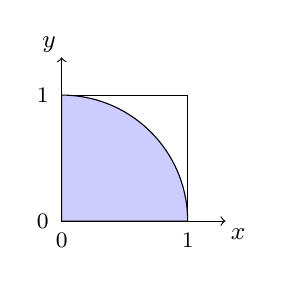
\begin{tikzpicture}[scale = 1.6]
\draw[thin] (0,0) -- (0,1) -- (1,1) -- (1,0) -- cycle; 
\filldraw[fill=blue!20!white, draw=black]
  (0,0) -- (1,0) arc (0:90:1) -- cycle;
\draw (0,\dd) node {\footnotesize $0$}; \draw (1,\dd) node {\footnotesize $1$};
\draw (\dd,0) node {\footnotesize $0$}; \draw (\dd,1) node {\footnotesize $1$};
\draw[->] (0,0) -- (1.3,0); \draw (1.4,-0.1) node {\small $x$};
\draw[->] (0,0) -- (0,1.3); \draw (-0.1,1.4) node {\small $y$};
\end{tikzpicture}
\end{myminipage}

\smallskip

The program below uses the bag-of-tasks pattern.  Each task is to generate
\SCALA{taskSize} pairs $(x,y)$ and to count how many satisfy $x^2+y^2 < 1.0$.
The controller sends a signal to a worker on |toWorkers| to tell it to perform
another task.  After |numTasks| such signals, it closes |toWorkers|, and each
worker sends its own count to the controller on |toController|.  The
controller than calculates the estimate of~$\pi$.   
%
\begin{scala}
object Pi{
  val taskSize = 400000 // Size of a single task.
  val numTasks = 200    // Number of tasks.
  val numWorkers = 8    // Number of workers.

  val toWorkers = new BuffChan[Unit](numWorkers)
  val toController = new BuffChan[Int](numWorkers)

  def worker = thread("worker"){
    val random = new scala.util.Random; var count = 0
    repeat{
      toWorkers?()
      for(i <- 0 until taskSize){
	val x = random.nextDouble(); val y = random.nextDouble()
	if(x*x + y*y < 1.0) count += 1
      }
    } // End of £repeat£ loop.
    toController!count
  }

  def controller = thread("controller"){
    for(i <- 0 until numTasks) toWorkers!()
    toWorkers.endOfStream()
    var count = 0
    for(i <- 0 until numWorkers) count += (toController?())
    println(4.0*count.toDouble/(taskSize*numTasks))
  }

  def system = controller || (|| ( for(i <- 0 until numWorkers) yield worker))

  def main(args: Array[String]) = run(system)
}
\end{scala}

We could have split the controller between two threads, and encapsulated each
into a separate object.

The above code gives each worker its own random number generator (RNG).  An
alternative is for the workers to share a single RNG.  However, my informal
experiments showed that the latter approach is about 20 times slower!  I think
the reason for this is that, when sharing, the state of the RNG has to be
copied to the cache of the relevant worker for each random number, and this is
slow.  When each worker has its own RNG, the state of that RNG will reside in
the worker's cache, and does not need to be reread from main memory.  

In fact, we should worry about whether sharing an RNG might constitute a race,
since the state of the RNG is updated for each random number.  However, it
turns out that the implementation does this in a thread-safe way.
\end{answerS}



%% If we let $n$ be the number of samples, then the number of samples that
%% satisfy the property $x^2+y^2<1$ has binomial distribution $Binom(n,\pi/4)$,
%% which has variance $n.\pi/4.(1-\pi/4)$, standard deviation
%% $\sqrt(n.\pi/4.(1-\pi/4))$, and so a standard deviation on the final result of
%% $4.\sqrt(\pi/4.(1-\pi/4)) / \sqrt n \approx 1.64 / \sqrt n$.  For $n = 10^6$, as
%% above, this is about $0.00164$.  This is consistent with the experimental
%% observation that the program is normally accurate to about two decimal places.


\begin{question}
Write a concurrent program to multiply two large |n| by |n|
matrices~|a| and~|b| together, storing the result in matrix~|c|.  You should
use the bag-of-tasks pattern.  You should consider what a suitable task
should be: remember that making a task too small will mean that workers spend
most of their time waiting to receive the next task.  \textbf{Optional:} carry
out some experiments to assess different sizes of tasks.
% You will probably want to represent each matrix by a two dimensional array.
% Such an array can be initialised in Scala using, e.g.:
% %
% \begin{scala}
% var a = new Array[Array[Int]](N,N);
% \end{scala}
% %
% The element in position $(i,j)$ can be accessed using \SCALA{a(i)(j)}.
\end{question}

%%%%%%%%%%%%%%%%%%%%%%%%%%%%%%%%%%%%%%%%%%%%%%%%%%%%%%%%%%%%

\begin{answerI}
It would be a mistake to take a task to be the calculation of a \emph{single}
entry in the result matrix.  That would make tasks too small (except, perhaps,
for very large values of~|n|), and lead to the communication channel being a
bottleneck.  Instead, we will take a task to involve calculating
\emph{multiple} entries in the result, |taskSize| entries in the code below.  

However, it's not clear whether a task should be part of a single row, or
multiple rows, i.e.~whether |taskSize| should be smaller or greater than~|n|.
The code below provides for both options: the type |Task| of tasks contains
two subtypes corresponding to the two options.

Most of the code is then straightforward.  Note that each worker can write
values directly into the result matrix~|c|: different threads write to
different entries in~|c| so there are no races.  Both the workers and the
server handle the different types of task in the obvious way.  The main
|apply| function runs the workers and server in parallel, and returns the
result array~|c|.
%
\begin{scala}
class MatrixMult(a: Array[Array[Int]], b: Array[Array[Int]],
             numWorkers: Int, taskSize: Int){
  private val n = a.size

  /** Array to store the result. */
  private var c = Array.ofDim[Int](n,n)

  trait Task

  /** The task to calculate entries [start..end) of row `row`. */
  case class SingleRowTask(row: Int, start: Int, end: Int) extends Task 

  /** The task to calculate rows [start..end). */
  case class MultiRowTask(start: Int, end: Int) extends Task

  /** Channel for sending tasks. */
  private val toWorkers = new SyncChan[Task] // (numWorkers)

  /** Calculate and store entry for c(i)(j). */
  private def calculate(i: Int, j: Int) = {
    var sum = 0; var k = 0
    while(k < n){ sum += a(i)(k)*b(k)(j); k += 1 }
    c(i)(j) = sum
  }

  /** A worker: repeatedly receive tasks, and calculate the relevant rows. */
  private def worker = thread{
    repeat{
      toWorkers?() match{
        case SingleRowTask(row, start, end) =>
          for(j <- start until end) calculate(row,j)
        case MultiRowTask(start, end) => 
          for(row <- start until end){
            var j = 0
            while(j < n){ calculate(row,j); j += 1 }
          }
      }
    }
  }

  private def server = thread{
    if(taskSize <= n){ // use SingleRowTasks.
      for(row <- 0 until n){
        var j = 0
        while(j < n){ 
          toWorkers!SingleRowTask(row, j, (j+taskSize) min n); j += taskSize
        }
      }
    }
    else{ // use MultiRowTasks.
      assert(taskSize%n == 0); val taskRows = taskSize/n // # rows per task.
      var row = 0
      while(row < n){
        toWorkers!MultiRowTask(row, (row+taskRows) min n); row += taskRows
      }
    }
    toWorkers.endOfStream()
  }

  def apply(): Array[Array[Int]] = {
    run((|| (for(i <- 0 until numWorkers) yield worker)) || server)
    c
  }
}
\end{scala}

%%%%%

Note that the computational cost of calculating each entry is $O(\sm n)$, so
the computational cost of each task is $O(\sm{taskSize} \times \sm n)$, and
the total computational cost is $O(\sm n^3)$.  By contrast, the total
communication cost is $O(\sm n^2 / \sm{taskSize})$.

The graph below gives the results of experiments to investigate the optimal
task size, using eight workers.  Each plot considers a particular value
of~|n|.  The x-axis considers different values for |taskSize| (with
$\sm{taskSize} \le \sm n^2$).  Each observation corresponds to $2^{21}/\sm n$
runs (this means, for a fixed value of |taskSize|, all plots have the same
communication cost).  The plots show the average time taken, with 95\%
confidence intervals, based on 50 observations.

\begin{center}
\begin{tikzpicture}
\begin{semilogxaxis}[
  ylabel = Time (ms),
  xlabel = Task size,
  log basis x=2,
  scaled ticks = false,
  legend pos = north west,
  ymax = 8000,
  height = 0.5\textheight,
  width = 0.8\textwidth
]
\addplot+[error bars/.cd, y dir=both,y explicit] coordinates {
  (16,3411.7514569200002) +- (0,13.35314203117615)
  (32,2069.33146884) +- (0,10.729978495813548)
  (64,1580.71169698) +- (0,12.187170381822089)
  (128,1331.7445018800001) +- (0,17.81049749071006)
  (256,1221.0753941199998) +- (0,14.036122865702522)
  (512,1200.1545826400002) +- (0,13.160170805411989)
  (1024,1224.52603058) +- (0,12.339814224799099)
  (2048,1180.51058504) +- (0,12.667749687921726)
  (4096,1238.1937666600002) +- (0,11.654862280558184)
};
\addlegendentry{$\sm n = 64$}
\addplot+[error bars/.cd, y dir=both,y explicit] coordinates {
  (16,2699.50312402) +- (0,12.525706223272508)
  (32,1492.46816324) +- (0,8.03041925064032)
  (64,1032.61340322) +- (0,9.65428666125068)
  (128,756.41274536) +- (0,9.451155367592488)
  (256,646.3791983) +- (0,8.007846740099064)
  (512,594.56514858) +- (0,8.834111329197311)
  (1024,574.4690993400001) +- (0,8.980969587496622)
  (2048,587.2721347) +- (0,8.86446678781081)
  (4096,592.8091398400001) +- (0,7.043147786939348)
  (8192,676.76904946) +- (0,6.514321066104861)
  (16384,896.66442712) +- (0,4.2726105430776595)
};
\addlegendentry{$\sm n = 128$}
\addplot+[error bars/.cd, y dir=both,y explicit] coordinates {
  (16,2585.2257487600004) +- (0,11.025475452786623)
  (32,1453.85767052) +- (0,8.03717703953275)
  (64,940.0082984) +- (0,6.807915846715892)
  (128,717.61791462) +- (0,9.03977554288971)
  (256,639.46824744) +- (0,9.995634498856198)
  (512,592.3433037799999) +- (0,8.50628975282786)
  (1024,562.1977136) +- (0,7.709808376242314)
  (2048,553.12491324) +- (0,9.561884603261213)
  (4096,557.26886086) +- (0,8.93908705796671)
  (8192,571.2262493200001) +- (0,10.331566458075345)
  (16384,618.6170808200001) +- (0,5.81423301764652)
  (32768,996.1779111000001) +- (0,5.534110197737152)
  (65536,1722.08606682) +- (0,4.427802338996753)
};
\addlegendentry{$\sm n = 256$}
\addplot+[error bars/.cd, y dir=both,y explicit] coordinates {
  (16,2466.5310879) +- (0,8.021048467527224)
  (32,1390.06749204) +- (0,8.237182191779926)
  (64,1193.3307740999999) +- (0,8.065081349160302)
  (128,1041.83938486) +- (0,9.241447251536886)
  (256,969.39207408) +- (0,8.718048838577854)
  (512,1035.4622452) +- (0,12.5560843960807)
  (1024,980.3836694400001) +- (0,10.649524436650921)
  (2048,922.15102602) +- (0,7.74849490705983)
  (4096,877.32535494) +- (0,5.03604122432872)
  (8192,868.437988) +- (0,6.90018903825376)
  (16384,874.77921678) +- (0,10.862135162173832)
  (32768,888.6167595) +- (0,12.722619106651159)
  (65536,1330.923144) +- (0,4.437714457552873)
  (131072,2488.52878918) +- (0,6.620712760530837)
  (262144,4814.394726979999) +- (0,12.967601048815668)
};
\addlegendentry{$\sm n = 512$}
\addplot+[error bars/.cd, y dir=both,y explicit] coordinates {
  (16,4369.8677981) +- (0,48.43900584396743)
  (32,3811.24042716) +- (0,21.672831073712185)
  (64,3882.9536471799997) +- (0,51.87991076642813)
  (128,3681.15564338) +- (0,27.973773946739687)
  (256,3752.1128576399997) +- (0,34.894632015903824)
  (512,3718.3242032) +- (0,25.092378003392046)
  (1024,3635.46097236) +- (0,26.3584784344136)
  (2048,3610.70516356) +- (0,16.29905651068537)
  (4096,3646.10937956) +- (0,30.033869221792447)
  (8192,3648.31660216) +- (0,19.710488335609607)
  (16384,3648.17540688) +- (0,20.541525935467135)
  (32768,3647.67361718) +- (0,21.210072979394173)
  (65536,3600.34809498) +- (0,33.545055491515576)
  (131072,3631.2190203) +- (0,29.952943406403094)
  (262144,6670.03208056) +- (0,38.08685982978708)
  (524288,12716.23585172) +- (0,76.26448592060504)
};
\addlegendentry{$\sm n = 1024$}
\end{semilogxaxis}
\end{tikzpicture}

\end{center}

Each of the plots has a fairly flat middle section, where the value of
|taskSize| makes little difference.  Typically, the fastest behaviour is where
each worker performs a few tasks; but the differences are often smaller than
the confidence intervals, so it's not possible to say definitively.

To the left, the program gets slower, as the communication cost dominates.
This is less of an issue when $\sm n = 1024$, because the computational cost
of each task is still quite large.

To the right, for most values of~|n|, the program gets slower as the number of
tasks is less than the number of workers!  However, for $\sm n = 64$, there is
little difference, as the savings on communication costs roughly balance the
extra computational cost for the workers that receive a task. 
\end{answerI}

%% It makes sense to define a \emph{task} to be the creation of several rows of
%% the result, say \SCALA{taskSize} rows.  
%% % The communication overhead is
%% % $\Theta(n/taskSize)$, so for large arrays, having a task as a single row
%% % (i.e.\ taking $taskSize=1$) would probably be too small a task (although the
%% % communication overhead of using a single row would be reasonably small
%% % compared to the $\Theta(N^3)$ computational cost).  
%% Taking a task to be a single entry in the result would be too small a task: it
%% would give a $\Theta(n^2)$ communication overhead.  Using a whole number of
%% rows (or columns) is easier to program than any other way of splitting up the
%% problem (e.g.\ into square regions).

%% There is no need for the workers to return any result to the controller: each
%% worker can write directly into the result array.  Note that since the tasks
%% write to disjoint parts of the result array, there are no race conditions. 

%% Here's my code:
%% %
%% \begin{scala}
%% class Matrix(a: Array[Array[Int]], b: Array[Array[Int]],
%%              numWorkers: Int, taskSize: Int){
%%   private val n = a.size

%%   /** Array to store the result. */
%%   private var c = Array.ofDim[Int](n,n)

%%   /** A task.  The pair (start,end) represents the task of calculating rows
%%     * [start..end). */
%%   private type Task = (Int,Int) 

%%   /** Channel for sending tasks. */
%%   private val toWorkers = new BuffChan[Task](numWorkers)

%%   /** A worker: repeatedly receive tasks, and calculate the relevant rows. */
%%   private def worker = thread{
%%     repeat{
%%       val(start,end) = toWorkers?()
%%       for(i <- start until end; j <- 0 until n){
%%         // Calculate value for c(i)(j)
%%         var sum = 0
%%         for(k <- 0 until n) sum += a(i)(k)*b(k)(j)
%%         c(i)(j) = sum
%%       }
%%     }
%%   }

%%   /** The controller: repeatedly allocate tasks of size taskSize. */
%%   private def controller = thread{
%%     var current = 0
%%     while(current < n){
%%       toWorkers!(current, current+taskSize min n)
%%       current += taskSize
%%     }
%%     toWorkers.endOfStream
%%   }

%%   /** calculate the product of a and b. */
%%   def apply(): Array[Array[Int]] = {
%%     val system = || (for(w <- 0 until numWorkers) yield worker) || controller
%%     run(system)
%%     c
%%   }
%% }
%% \end{scala}


%% %
%% %% \begin{scala}
%% %% class Matrix(a: Array[Array[Int]], b: Array[Array[Int]], numWorkers: Int, taskSize: Int){
%% %%   private val n = a.size

%% %%   /** Array to store the result. */
%% %%   private var c = Array.ofDim[Int](n,n)

%% %%   /** A task.  The pair (start,end) represents the task of calculating rows [start..end). */
%% %%   private type Task = (Int,Int) 

%% %%   /** Channel for sending tasks. */
%% %%   private val toWorkers = OneMany[Task]

%% %%   /** A worker: repeatedly receive tasks, and calculate the relevant rows. */
%% %%   private def worker = proc{
%% %%     repeat{
%% %%       val(start,end) = toWorkers?()
%% %%       for(i <- start until end; j <- 0 until n){
%% %% 	// Calculate value for c(i)(j)
%% %% 	var sum = 0
%% %% 	for(k <- 0 until n) sum += a(i)(k)*b(k)(j)
%% %% 	c(i)(j) = sum
%% %%       }
%% %%     }
%% %%   }

%% %%   /** The controller: repeatedly allocate tasks of size taskSize. */
%% %%   private def controller = proc{
%% %%     var current = 0
%% %%     while(current < n){
%% %%       toWorkers!(current, current+taskSize min n)
%% %%       current += taskSize
%% %%     }
%% %%     toWorkers.close
%% %%   }

%% %%   /** calculate the product of a and b. */
%% %%   def apply(): Array[Array[Int]] = {
%% %%     run(|| (for(w <- 0 until numWorkers) yield worker) || controller)
%% %%     c
%% %%   }
%% %% }
%% %% \end{scala}

%% %% I ran some informal experiments based around the following function.  The
%% %% ``warm up'' part is to avoid the effects of JIT compilation.
%% %% %
%% %% \begin{scala}
%% %%   /** Measure times for different task sizes, for matrices of size n and
%% %%     * numWorkers worker threads. */
%% %%   def timingTest(n: Int, numWorkers: Int) = {
%% %%     // # reps; chosen to spend ~3s per task size
%% %%     val reps = (300L*Million*numWorkers/(n.toLong*n*n)).toInt
%% %%     println("reps = "+reps)
%% %%     // Warm up
%% %%     for(_ <- 0 until reps){
%% %%       val a = randomArray(n); val b = randomArray(n)
%% %%       val c = new Matrix(a, b, numWorkers, 2)()
%% %%     }
%% %%     println("starting")
%% %%     for(taskSize <- 1 until 10){
%% %%       var elapsed = 0L
%% %%       for(_ <- 0 until reps){
%% %%         val a = randomArray(n); val b = randomArray(n)
%% %%         val start = System.nanoTime
%% %%         val c = new Matrix(a, b, numWorkers, taskSize)()
%% %%         elapsed += System.nanoTime-start
%% %%       }
%% %%       println(taskSize+"\t"+elapsed/Million+"ms")
%% %%     }
%% %%   }
%% %% \end{scala}
%% %

%% I ran some informal experiments, considering different values of~|n|, and
%% different task sizes.
%% For small values of |n| (around 200) a task size of 2 was often best; with
%% smaller tasks, the $O(\sm n^2/\sm{taskSize})$ communication overhead meant
%% that the controller was a bottleneck.  For larger values of |n|, a task size
%% of~1 was best; each task has $O(\sm n^2)$ computational cost, which is
%% sufficiently large that the controller is not a bottleneck; and having more
%% tasks gives better load balancing.  It might be interesting to run experiments
%% with smaller tasks, say to calculate part of a row of the result.
%% \end{answer}
 % Matrix multiplication Q (sheet 1.5)

\framebox{?} Count \# common values (sheet 1.6) --- I think the best way to
solve this problem is to use a shared hash table; but that will appear later
in the book. 

\framebox{?} Maximum in array.




